\documentclass[letterpaper]{report}

% packages to include additional functionality
\usepackage{makeidx}         % allows index generation
\usepackage{graphicx}        % standard LaTeX graphics tool
\usepackage{multicol}        % used for the two-column index
\usepackage[bottom]{footmisc}% places footnotes at page bottom
\usepackage{wrapfig} % for wrapping images with text
\usepackage{color} % for coloring links
\usepackage{fancyvrb}
\usepackage{listings}
\usepackage{verbatim}
\usepackage{fixltx2e}
\usepackage{hyperref}%for including URL
%Start Margins
\addtolength{\oddsidemargin}{-.875in}
\addtolength{\evensidemargin}{-.875in}
\addtolength{\textwidth}{1.75in}
\addtolength{\topmargin}{-.885in}
\addtolength{\textheight}{1.95in}
%End Margins

\begin{document}

\renewcommand{\thesection}{\arabic{section}}

\author{Bharath Kongara	}
\title{CS 751: Assignment 2}

\date{Spring 2015}

% note that this special command is part of the document class
% and, in addition to creating the title page, also inserts the 
% current date on the page
\maketitle

\tableofcontents
\newpage

% include other tex files so we don't have one huge document to scroll through




\section{Problem 1}
\label{part1}

Demonstrate that you know how to use "curl" well enough to
correctly POST data to a form.  Show that the HTML response that
is returned is "correct".  That is, the server should take the
arguments you Posted and build a response accordingly.  Save the
HTML response to a file and then view that file in a browser and
take a screen shot.

\subsection{Solution}

The following steps were taken to become familiar with curl:
\begin{enumerate}
	\item Executed the simple curl command for couple of websites in order get the source code of that particular page and learned how to inspect the POST method in form tags.
\begin{verbatim}
	curl www.cs.odu.edu	
\end{verbatim}
	\item Created simple php login page where there are 2 text fields in a form tag, the data entered in the text fields are submitted to the next page through POST method and displayed there. 
	\item The text fields names are "uname" and "password" 
	\item With the options -d in curl we can send the arguments in a POST request to the HTTP server, like a browser does when a user had filled in an HTML form and presses the submit button.
	\item Option -F in curl is similar to -d option, in addition enables  uploading of binary files. 
\end{enumerate}

\subsection{Code Listing}
Here are the two PHP pages to which the curl command is used 
\subsubsection{loginform.php}
\lstinputlisting[language=PHP, breaklines=true]{loginform.php}
\newpage
\subsubsection{login.php}
\lstinputlisting[language=PHP, breaklines=true]{login.php}
\subsubsection{Methodology }
\begin{enumerate}
\item  The following command is used to post data through curl
\begin{verbatim}
	curl -F u_name=mallika -F password=mallika1 www.cs.odu.edu/~mkogatam/fall14/cs595/login.php
	OR
	curl -d u_name=mallika -d password=mallika1 www.cs.odu.edu/~mkogatam/fall14/cs595/login.php
\end{verbatim}
\item Here the argument "mallika" and "mallika1" are posted as user name and password respectively to server through a curl command. 
\item When -d option is used in curl it will send the parameters mentioned in the command to a HTTP server through a POST request and gets the output. 
\item If the text field name is given wrong then it does not pass any value to the HTTP server. 
\end{enumerate}
\newpage
\subsection{Results}

Here is the HTML response created from the above command. 

\lstinputlisting[language=HTML, breaklines=true]{part1_response.htm}

\begin{figure}[ht]    
    \begin{center}
        \includegraphics[scale=0.60]{part1_response.png}
        \caption{Response for the curl command}
        \label{fig:X-distribution}
    \end{center}
\end{figure}

\section{Question 2}
\label{part2}
\begin{itemize} 
\item Using the pages from Q1 (A4), download all TimeMaps (including TimeMaps with 404 responses, i.e. empty or null TimeMaps) 
\begin{itemize}
\item Upload all the TimeMaps to github
\end{itemize}

\item Build a CDF for \# of mementos for each original URI (i.e., x-axis = \# of mementos, y-axis = \% of links)
\item See: \url {http://timetravel.mementoweb.org/guide/api/} 

\end{itemize}
\subsection{Solution}
\begin{itemize}
 \item I used `timelapse'\cite{timelapse} library to retrieve TimeMaps of each of the URIs.
 \item `timelapse'\cite{timelapse} library extracts memento created date along with memento.
 \item Out of 9,800 URIs, TimeMaps are retrieved for 8200 which includes empty files.
 \item I ran multiple instances to retrieve TimeMaps as aggregator was taking time.
 \item Few times retrieval stopped because of request time out error. I waited for a few minutes before running it again.
 \item I have uploaded TimeMaps of each of the URIs to Github.
\end{itemize}

\lstinputlisting[language=Python,breaklines = true,frame=single,caption={Python program to retrieve TimeMap of each of the URIs}, label=lst:q1-1,captionpos=b,numbers=left,showspaces=false,showstringspaces=false,basicstyle=\footnotesize]{getmaps.py}

\begin{figure}[ht]
	\begin{center}
		 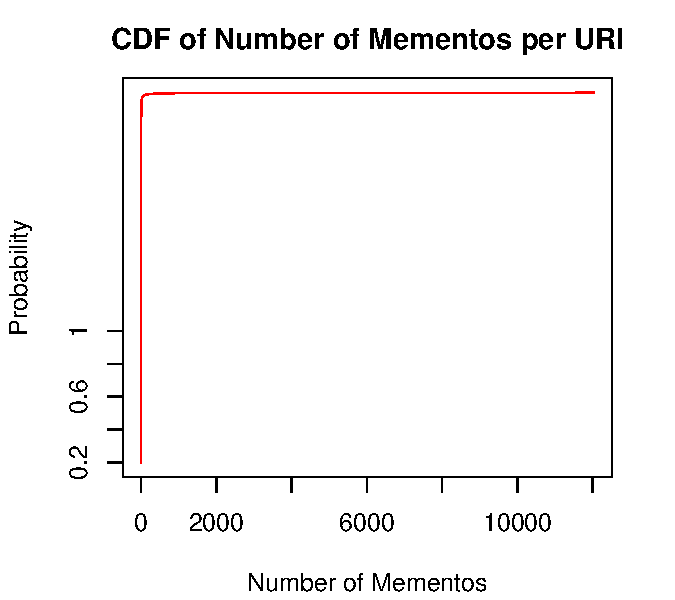
\includegraphics[scale=0.60]{memento_counts}
		  \caption{CDF of Number of Memento count per URI}
	 \end{center}
\end{figure}
\newpage




\bibliographystyle{plain}
\bibliography{assignment2}
\nocite{*}

\end{document}

